\documentclass[11pt]{article}
\usepackage{geometry}                
\geometry{letterpaper}                   

\usepackage{graphicx}
\usepackage{amssymb}
\usepackage{epstopdf}
%\usepackage{natbib}
\usepackage{amssymb, amsmath}
\usepackage{here}
\usepackage{subfigure}
\usepackage{hyperref}
\DeclareGraphicsRule{.tif}{png}{.png}{`convert #1 `dirname #1`/`basename #1 .tif`.png}
\usepackage{color}
\newcommand{\warn}{\textcolor{red}}


\usepackage[
    backend=biber,
    style=ieee
    ]{biblatex}
\addbibresource{ref.bib}

%\title{Title}
%\author{Name 1, Name 2}
%\date{date} 

\hypersetup{
    colorlinks=true,
    linkcolor=blue,
    filecolor=magenta,      
    urlcolor=blue,
    pdftitle={SZR Model},
    pdfpagemode=FullScreen,
}

\begin{document}



\thispagestyle{empty}

\begin{center}
\includegraphics[width=5cm]{ETHlogo.eps}

\bigskip


\bigskip


\bigskip


\LARGE{Complex Social Systems:\\ }
\LARGE{Modeling Agents, Learning, and Games HS2021\\}

\bigskip

\bigskip

\small{Project Report}\\

\bigskip

\bigskip

\bigskip

\bigskip


\LARGE{\textbf{Virtual Zombie Pandemic on Lattice:}}\\
\LARGE{\textbf{Critical Phenomenon and Reinforcement Learning}}\\

\bigskip

\bigskip

\bigskip

\LARGE{Noureddine Gueddach\\
       Chang Sun\\
       Yifeng Wang\\
       Rong Zhang
       }



\bigskip

\bigskip

\bigskip

\bigskip

\bigskip

\bigskip

\bigskip

\bigskip

Zurich\\
Dec 2021\\

\end{center}



\newpage

%%%%%%%%%%%%%%%%%%%%%%%%%%%%%%%%%%%%%%%%%%%%%%%%%

\newpage
\section*{Agreement for free-download}
\bigskip


\bigskip


\large We hereby agree to make our source code for this project freely available for download from the web pages of the SOMS chair. Furthermore, we assure that all source code is written by ourselves and is not violating any copyright restrictions.

\begin{center}

    \bigskip


    \bigskip


    \begin{tabular}{@{}p{3.3cm}@{}p{6cm}@{}@{}p{6cm}@{}}
        \begin{minipage}{3cm}

        \end{minipage}
         &
        \begin{minipage}{6cm}
            \vspace{2mm} \large Noureddine Gueddach

            \vspace{\baselineskip}
            \large Chang Sun
        \end{minipage}
         &
        \begin{minipage}{6cm}
            \vspace{2mm} \large Yifeng Wang

            \vspace{\baselineskip}
            \large Rong Zhang
        \end{minipage}
    \end{tabular}


\end{center}
\newpage

%%%%%%%%%%%%%%%%%%%%%%%%%%%%%%%%%%%%%%%



% IMPORTANT
% you MUST include the ETH declaration of originality here; it is available for download on the course website or at http://www.ethz.ch/faculty/exams/plagiarism/index_EN; it can be printed as pdf and should be filled out in handwriting


%%%%%%%%%% Table of content %%%%%%%%%%%%%%%%%

\tableofcontents

\newpage

%%%%%%%%%%%%%%%%%%%%%%%%%%%%%%%%%%%%%%%



\section{Abstract}
This report studies a virtual zombie pandemic using the SZR (survivor, zombie, removed) model. We first solved the analytical solution for the SZR model and discussed the computer simulation method. The system behavior and critical points for the SZR model and its derivatives are discussed in detail. Finally, we use a reinforcement learning algorithm to train the agents to move in order to depict the behavior of zombies and survivors dynamically.

\section{Individual contributions}

Gueddach Noureddine studied the critical point on the hexagonal lattice, before working on the mitigation strategies using reinforcement learning.

Chang Sun proposed the Modified SZR model and implemented the (Modified) SZR model with the ``contact tracing'' algorithm. He also performed the critical point-occupancy study for the MSZR / SZR model on a square lattice.

Yifeng Wang is the main contributor for drafting and editing this written report. His other contribution is showing the analytical solutions and verifying the code of other exploratory studies. 

Rong Zhang implemented the queue-bond algorithm and studied the relation between the critical point of the SZR model and the sparsity with it.

\section{Introduction and Motivations}
Though it has never been confirmed (to the best of our knowledge), zombie pandemic outbreak has proven themselves to be an interesting field to investigate in recent years. As a familiar topic to the public, many have investigated such virtual pandemic and modeled it \cite{casestudy} \cite{math_model_attack} \cite{bayesian} \cite{emotion}. While some focus on the strategies and probabilities of survival \cite{survival}, or variables \cite{emotion} in the zombie pandemic itself, it is shown that the zombie models can be made in parallel to other phenomenons (e.g., rumors \cite{rumor}). Besides, though the pandemic itself is virtual, it may grant us valuable insights regarding the real pandemics \cite{eval}.

In our exploratory study, we investigated the SZR model introduced in \cite{Zombies} and its derivatives. The SZR model introduced in \cite{Zombies} is similar to the SIR model, except for the distinct behavior of the agents. Due to this difference, the SZR model has advantages in describing other scenarios that depart from the conventional disease (i.e., bacteria in cells, rumor spread in villages, or even zombie pandemic outbreaks). We take zombie pandemic outbreaks as a general scenario to study the SZR model in detail. We start with a simple square-shape pixel; then, we advance to hex pixel. We will cover the critical behavior of the model and explore its correlation with $\alpha$. We will also discuss the mitigation strategies for agents. 

\section{Description of the Model}
We should give a quick recap on SIR model first. SIR model is governed by three differential equations which states the time evolution of a given variable (i.e. S, Z, and R). S stands for the stock of susceptible population, I is the stock of infected, and R is the stock of removed population.
\begin{align}
    \dot{S} & = -\frac{\beta IS}{N},           \\
    \dot{I} & = \frac{\beta IS}{N} - \gamma I, \\
    \dot{R} & = \gamma I.
\end{align}
Since $N$ is just the normalization constant, exploring other parameters inside the differential equations is worthwhile. Unsurprisingly, the ratio of two parameters $R_0 = \frac{\beta}{\gamma}$ needs special attention, as it can be used to derive the expected number of new infections, which is called the basic reproduction ratio. With the simple SIR model as a foundation, numerous models have been derived to describe the behavior of various systems. The most phenomenological use of instance is an epidemic disease and prey-predator biological system. Unfortunately, the SIR model is computationally intensive due to the disadvantage of not admitting to closed-form analytical solutions, especially on a large grid.

To address the shortcoming of the SIR model, we introduce the SZR model, which is abbreviated for ``survivors'', ``zombie'', and ``removed''. The SZR model is inspired by the study of zombie break out in such a scenario that zombies will ``bite'' survivors and survivors will ``kill'' zombies. Fortunately, our SZR model can be solved analytically, giving more opportunities to explore its applications. The key distinction from the SIR model is that the state turning rate (from S to Z or Z to R) is density-dependent rather than frequency-dependent. At a given site, the turning rate is solely dependent on the number of zombies and survivors interacting. Another interesting fact is that the R in the SZR model is non-reversible because dead zombies cannot be brought back to life either into a human or a zombie form.

\begin{align}
    \dot{S} & = -\beta SZ,        \\
    \dot{Z} & = (\beta-\kappa)SZ, \\
    \dot{R} & = \kappa SZ.
\end{align}

Besides the zombie breakout scenario, the SZR model has many realistic applications, such as virus attacks on human cells, forest fire progression, and rumor spreading in crowds.

\subsection{Analytical solution}
\label{sec:analy}
We will discuss the analytical solution of our SZR model; with these, we can calculate and predict the final states given the initial conditions without going into a stochastic process. First, the equation can be cast into a non-dimensional form, by replacing the dimensionless time parameter $\tau=t\beta N$ and the dimensionless so-called virulence $\alpha=\kappa/\beta$ \cite{Gillespie}.
\begin{align}
    \frac{\dot{S}}{d\tau} & = - \frac{SZ}{N},         \\
    \frac{\dot{Z}}{d\tau} & = (1-\alpha)\frac{SZ}{N}, \\
    \frac{\dot{R}}{d\tau} & = \alpha\frac{SZ}{N}.
\end{align}
Then, with the assumption that the initial conditions are $R(0)=0$, $Z_0=Z(0)$, and $S_0=S(0)$. We have the analytical solution as
\begin{align}
    P       & \equiv Z_0 + (1-\alpha)S_0,                           \\
    \mu     & \equiv \frac{S_0}{Z_0}(1-\alpha) = \frac{P}{Z_0} - 1, \\
    f(\tau) & \equiv \frac{P\mu}{e^{\tau P/N}+\mu},                 \\
    Z(\tau) & = P - f(\tau),                                        \\
    S(\tau) & = \frac{f(\tau)}{1-\alpha}.
\end{align}
To illustrate more, the sign of function $P$ indicates whether human will win or not. The final state has the property that
\begin{align}
    Z_\infty & = Z_0 + (1-\alpha)S_0, \text{(if human wins)}       \\
    S_\infty & = S_0 -\frac{Z_0}{\alpha-1} \text{(if zombie wins)}
\end{align}

\section{Implementation}
\subsection{Stochastic process and Gillespie algorithm}
In the last sections, toy models are on the basis of continuous simulation, so the number of agents in any state can have decimals. While continuous simulation is computationally efficient and accurate when all S and Z states are comparable, the stochastic simulation needs to be implemented to better emulate the entire process, especially at the beginning of the process, where the first zombie has the possibility of being eliminated, corresponding to the no-breakout scenario, or in the end, few survivors can hold their lines with removed states in between zombies. All of such exceptional scenarios have to be included in the progression of the system by SZR model. Thus, our codes are based on discrete stochastic simulations.

\subsection{Queue-bond}
\label{queue-bond}
Besides, we can further explore the system by localizing SZR states to each 2D pixel. Only one type of state can occupy a site, and the pixel can interact with neighbor pixels according to the SZR differential equations.

To be more efficiently simulate the evolution of the ``killing'' and ``biting'' processes, rather than calculating each individual ``fighting'' across the edge of the pixel. The key is to record only the bond between S and Z states which is the connection between local survivors and zombies. At each time step, we randomly choose a bond with a human site being infected with the probability of $1/(1+\alpha)$ and a zombie site being killed with the probability of $\alpha/(1+\alpha)$.

\subsection{Modified SZR Model}
A modified version derived from the original SZR model is proposed for on-lattice simulation as a more ``realistic'' situation to include the on-site density-dependent for killing and biting rate. The differential equations of the modified model are expressed in \ref{MSZR_difeq}, referred to as the Modified SZR (MSZR). This model is considered a more realistic case as zombies do not ``bite faster'' because there are more humans around it, contrasting to the original SZR model. Also, in contrast to \cite{Zombies}, we allow multiple people on the same grid point in a lattice. The number of people on one grid point is denoted as occupancy. Each grid point is connected to $5$ grid points in the square lattice: its four neighbors and itself. When the occupancy is precisely $1$, this is equivalent to the square model proposed in \cite{Zombies}. Consequently, the number of vertices for the modified model is $4n+(n-1)=(5n-1)$ ($4n$ neighbors in adjacent grid points and $(n-1)$ neighbors on the same grid point), where $n$ is the occupancy.

\begin{align}
    \dot{S} & = -\beta Z,         \\
    \dot{Z} & = \beta Z-\kappa S, \\
    \dot{R} & = \kappa S.
    \label{MSZR_difeq}
\end{align}

\subsubsection{Contact Tracing}
The queue-bond algorithm is no longer valid with the modified model: the probability of having state transition on each bond is not equal. Hence, instead, we used a contact tracking algorithm, which keeps track of all grid points having none-zero $Z$, with non-zero $S$ in its neighborhood, where $S$ in such grids is denoted $S_{ij}^*$. The vice versa is performed for Z. For each new step. There is a probability of $K/(K+B)$ that a zombie is killed, with $K=\kappa\sum S_{ij}^*$ and $B=\beta\sum Z_{ij}^*$. Then, a weighted sample, with weight being ${S_{ij}^*}$ or ${Z_{ij}^*}$, is performed to choose which grid initiates the action (kill or bite), and a random neighbor of it will receive the action. The contact list of the grids having state modified and all its neighbor's state in the contact tracing lists are updated accordingly.\par

The algorithm described is checked on the vanilla SZR model as a safety measure. With replacing the probability of kill to $\kappa/(\kappa+\beta)$ and weight being ${S_{ij}^*\cdot Z_{<ij>}}$ or ${Z_{ij}^*\cdot S_{<ij>}}$, where $Z_{<ij>}$ or $S_{<ij>}$ denotes the total number of $Z$ or $S$, respectively, in the neighborhood of grid point $(i,j)$, this algorithm produces a similar critical point for the SZR model with an occupancy of $1$. As the efficiency of this algorithm is one order slow than the one proposed in \cite{Zombies}, we used a smaller lattice of $256\times 256$ size for critical point search.

\section{Critical Point}
%\warn{[ToDo: introduce critical point, self-similar pattern ...]}
According to \cite{Zombies}, when the inverse virulence $\alpha$ is small, the zombie outbreak will cover the whole lattice. When $\alpha$ is large, humans will be able to contain the zombie outbreak before it reaches the boundary of the lattice. At the critical point $\alpha_{c}$, the zombie outbreak reaches the boundary, but forms a self-similar pattern, or fractal. Although the random fractal is not transformed to itself by scaling like the Sierpinski carpet, the probability distribution of the size of the cluster should satisfy $P(s) = f P(s/B)$, where $B$ denotes the scaling factor.\\

This phenomenon is closely related to the renormalization group, which has also been applied to theoretical condensed matter physics and high-energy physics. In the context of condensed matter physics, for example, the renormalization group transformation is applied to deriving the relations between the critical exponents and computing the critical point numerically of the 2D Ising model, which describes the transition from paramagnetism to ferromagnetism in many materials. By requiring the partition function to be equivalent before and after replacing blocks of spins on the Ising lattice by a single spin according to some predefined rules, the effective coupling between spins can be determined, so does the critical temperature. In the context of high-energy physics, this phenomenon is understood as a result of coarsifying the details of a theory. When theory goes to higher energy, the measurement resolution is increased, which implies subtle structure will appear. However, some sub-structures will be repeating themselves in the larger picture, just like snowflakes. In quantum field theory, the critical point is defined as the fix-point of the beta function at which the theory is scale-free. No matter how many higher-order expansions of correlation function we include, analogous to increasing scope resolution, the theory is still renormalizable. This is because the counter-terms precisely cancel the divergent terms at the critical point. Such scale-invariant property is why theorists shall be sensitive to whether the system admits a critical point. Analogously, in our case, the critical point is the $\alpha$ at which the SZR system has no natural scale. Pictorially, the pattern of survivors or zombies will be repetitive on small and large scales.

%This phenomenon has been discovered in many fields in physics, for instance, the phase transition of a crystal system and even the renormalization group for high-energy physics. This phenomenon is understood as a result of coarsifying the details of a theory. When theory goes to higher energy, the measurement resolution is increased, which implies subtle structure will appear. However, some sub-structures will be repeating themselves in the larger picture, just like snowflakes. In quantum field theory, the critical point is defined as the fix-point of the beta function at which the theory is scale-free. No matter how many higher-order expansions of correlation function we include, analogous to increasing scope resolution, the theory is still renormalizable. This is because the counter-terms precisely cancel the divergent terms at the critical point. Such scale-invariant property is why theorists shall be sensitive to whether the system admits a critical point. Analogously, in our case, the critical point is the $\alpha$ at which the SZR system has no natural scale. Pictorially, the pattern of survivors or zombies will be repetitive on small and large scales.

\subsection{Critical Point Search}

The search of critical points is based on the self-similarity of the percolation clusters at the critical point and the scaling behavior close to the critical point. Numerical experiments have support the assumption that the distribution of the cluster size $n_{s}$ near the critical point is proportional to $s^{-\tau} f((\alpha - \alpha_{c})s^{\sigma})$, where $f$ is an analytic function. \cite{Stauffer2018} The self-similarity of the percolation cluster at critical point requires $n_{s} \propto s^{-\tau}$. Therefore, after Taylor expansion, the
the probability that a cluster is greater than $s$ in size is related to the model parameter, in this case, the inverse virulence $\alpha$, by
\begin{align}
    P_{\geq s} \sim s^{2 - \tau} (A + B (\alpha - \alpha_{c})s^{\sigma}),
    \label{eqn:slope-alpha}
\end{align}
where $\tau$ and $\sigma$ are critical exponents. An approximation to the critical point is found if the $s^{\tau - 2} P_{\geq s}$ versus $s^{\sigma}$ curve has zero slope within the statistical uncertainty. The critical point is determined by linear fitting of the $\text{slope} - \alpha$ curve. The slope of the $s^{\tau - 2} P_{\geq s}$ is determined by linear fitting to the simulation data. As the Equation \ref{eqn:slope-alpha} is valid for large cluster and our simulation is on a finite lattice, we avoid the artifacts arising from the finite periodic lattice by fitting to data of clusters of moderate size.\\



%\warn{[ToDo: explain why we can use sigma and tau for 2D percolation](working on it...)}
\cite{Zombies} has shown that the percolation exponent $\tau$ for the vanilla SZR model is the same as that for 2D random percolation. The critical exponent $\tau$ for 2D random percolation describes the distribution of the size of clusters formed by randomly occupying a 2D lattice site, which also describes the distribution of the size of clusters formed by burned trees in the forest fire model. The study of 2D random percolation shows that \cite{Stauffer2018} the critical exponents depends on the dimensionality of the lattice, but not the detail of the lattice, i.e. the critical exponents of 2D square or hexagonal lattices are identical, but different from that for 3D lattices, or Bethe lattices, etc. As the study of sparsity is an effective reduction of coordination number, we expect the critical exponents remain unchanged. In fact, we will see the SZR model reduces to the forest fire model at the critical sparsity, which further justifies our choice of 2D percolation exponent. Figure \ref{fig:p-geq-s-50000-1024} shows a frugal replication of the result in \cite{Zombies}.  For our study of the critical point of a square lattice with low occupation number, Figure \ref{fig:p-geq-s-0.35} shows a similar behavior as the vanilla SZR model, supporting our choice of the percolation exponents for the study of sparsity.\\

\begin{figure}[H]
    \centering
    \includegraphics[width=0.9\textwidth]{fig/P_geq_s_50000_1024.pdf}
    \caption{Red line: a line with $\text{slope} = 2 - \frac{187}{91}$. Blue dots: cumulative cluster size distribution of 50000 simulations on $1024 \times 1024$ square lattice of the vanilla SZR model at the critical point $\alpha_{c} = 0.43734613$.\cite{Zombies}}
    \label{fig:p-geq-s-50000-1024}
\end{figure}

\begin{figure}[H]
    \centering
    \includegraphics[width=0.9\textwidth]{fig/P_geq_s_alpha0.35.pdf}
    \caption{Red line: a line with $\text{slope} = 2 - \frac{187}{91}$. Blue dots: cumulative cluster size distribution of 50000 simulations on $1024 \times 1024$ square lattice of the SZR model with $\text{sparsity} = 0.35$ at the critical point $\alpha = 0.0805$.}
    \label{fig:p-geq-s-0.35}
\end{figure}

In order to search for critical points of the low-occupancy lattices, bootstrapping is performed to determine the uncertainty of the slope, i.e., the linear fit is performed to samples obtained from resampling without replacement from the simulation. The standard deviation of 100 sets of samples from resampling is taken as the uncertainty of the slope estimate. We start from two initial $\alpha$. We evaluate the slope and perform a linear fit to obtain a new critical point estimation. Then the slope of the new $\alpha$ is evaluated and added to the data points for the linear fit. Once the magnitude of the estimated slope is smaller than the uncertainty, we quadruple the sample size for the measurement of cluster size until the maximum allowed sample size is reached, which is set to be 64000. The simulations are performed on $1024 \times 1024$ square lattice. Since the accuracy of our critical point is sufficient for the phase diagrams, we did not perform a rigorous uncertainty quantification on the critical points. However, such analysis can be performed by error propagation based on the linear fit.\\



The critical point for high-occupancy lattices are performed in a ``quasi'' binary-search way, based on the scaling postulate: One first set an upper bound $\alpha_h$ and a lower bound $\alpha_l$ before the search. In a new iteration, $\alpha$ is initialized by $(\alpha_h+\alpha_l)/2$. The algorithm then simulates the same lattice with different random seeds for $1024$ times, and a linear fit is performed with $x=s^\sigma$ and $y=s^{\tau-2}P_{\geq s}$, on where the curve is on a plateau. By the scaling postulate, this slope is $0$ when $\alpha=\alpha_c$. Hence, when the slope is smaller than $0$, $\alpha_h\leftarrow\alpha$, or $\alpha_l\leftarrow\alpha$ otherwise. When $|\mathrm{slope}|<3\sigma_{fit}$, the iteration breaks, and current $\alpha$ is deemed to be $\alpha_c$. However, notice that this algorithm diverges from the conventional binary search in one way: when the slope changes in an unexpected way after updating one boundary, the last change in the boundary of the opposite direction will be undone. (e.g., if the slope decreases after decreasing $\alpha_h$, the last increment of $\alpha_l$ be undone.) The resolution of $\alpha_c$ obtained this way is inferior to the one used for low-occupancy lattices, but is used based on performance considerations.

\begin{figure}[H]
    \centering
    \subfigure[Square lattice]{
        \includegraphics[height=0.4\textwidth]{fig/hex_expl_1.pdf
        }
    }
    \subfigure[Hexagonal lattice]{
        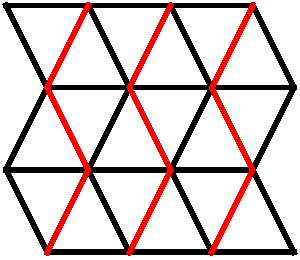
\includegraphics[height=0.4\textwidth]{fig/hex_expl_2.pdf
        }
    }
    \caption{Bond mapping from square lattice to hexagonal lattice}
    \label{fig:sqrt2hex}
\end{figure}

\subsection{Results and Discussions on Critical Point Dependence}

We extend the same methodology to the hexagonal lattice in order to verify that the latter belongs to the same universality class as the square lattice. To do so, we compute the new critical point $\alpha_c$ and examine it; we compute the probabilities of sites being in a cluster of size at least $s$ (x-axis in Figure~\ref{fig:hex_critical_point} b). The points forming a line on a log-log plot with the same slope (2 - $\tau$) as the square lattice indicates that it follows the same power law and hence verifies our prediction ($\tau = 187/91$ is given by percolation theory). To actually compute the critical point, we follow the strategy described in section \ref{queue-bond} and we find a value of $\alpha_\text{c, hexagonal} \approx 0.527825$ which is higher than that of the square lattice ($\alpha_\text{c, square} = 0.43734613$). The method of embedding the hexagonal lattice in a square lattice is shown in Figure~\ref{fig:sqrt2hex}, where the hexagonal lattice is shown on the right and the square lattice is shown on the left.\\

Some of the results for the critical point are shown in Figure~\ref{fig:hex_critical_point}: (a) shows $s^\sigma$ plotted against $s^{\tau-2}P_{\geq s}$ ($\sigma=36/91$ also given by percolation theory). A flat tangent to the graph indicates a scale-invariant (clusters of different sizes are equally likely), which in turn indicates that we are at the critical point. Indeed, for instance, with $\alpha > \alpha_c$, we get a negative slope (and hence fewer large clusters, i.e., humans win) and vice-versa. As can be seen in (c), various $\alpha$'s become almost indistinguishable at the precision we operate. To get more precision, we use the graph in (d); notice that our critical point $\alpha_c$ has a slope of almost zero (slope k = $7.1565 \times 10^{-7}$). Finally, (e) shows the resulting lattice with the computed critical point after an outbreak.\\

Besides, studies on the critical point dependence on the sparsity/occupancy are done, and the results are presented in Figure~\ref{fig:alphac-p} and Figure~\ref{fig:alphac-o}. \\

\begin{figure}[H]
    \centering
    \includegraphics[width=0.8\textwidth]{fig/sparsity_phase.pdf}
    \caption{Critical point - Sparsity, SZR model}
    \label{fig:alphac-p}
\end{figure}

Sparsity is defined as the probability that a lattice site is empty. The empty state is effectively the same as the removed state, except that it is not considered to be a part of the infected cluster, unlike the removed state. In the hypothetical zombie outbreak scenario, the empty sites play the role of randomly placed firewalls. The critical point decreases with increasing sparsity until it reaches zero at $p = 0.407$ \cite{comphys2019}, which is the percolation threshold of the forest fire model.\\

The forest fire model describes the scenario where each site on a lattice is occupied with trees at a probability. At the onset of the simulation, there is only one burning tree. In each time step, all the nearest neighbors occupied by trees of a burning tree catch fire, and all the burning trees burn out. In this way, at the end of the simulation, the forest fire will cover the whole connected cluster. The percolation threshold of the forest fire model is the density of the trees where an infinite cluster starts to appear on an infinite lattice.\\

\begin{figure}[H]
    \centering
    \includegraphics[width=0.6\textwidth]{fig/Critical_Occupancy_SZR.pdf}
    \caption{Critical Point - Occupancy, SZR model\\
        An averaged occupancy $n$ is obtained by letting the probability of each grid point having occupancy of $\lfloor n\rfloor$ be $p$, and the probability of having an occupancy of $\lceil n\rceil$ be $(1-p)$, with $p=n-\lfloor n\rfloor$. The hexagonal equivalent point is evaluated by the degree of vertices (individuals): With an occupancy of $n|n\in\mathbb{N}_*$, the degree of vertices is $(5\cdot n-1)$. Hence, with the hexagonal model at an occupancy of $1$, as all its vertices have a degree of $6$, it is expected to be equivalent to a square model with an occupancy of $1.4$. More details of this hexagonal model are described in section \ref{hex}.
        \label{fig:alphac-o}
    }
\end{figure}

Though it looks that the Figure~\ref{fig:alphac-o} critical point is nearly linear dependent on the occupancy/sparsity, the Figure~\ref{fig:alphac-p} showed that the relationship is not exact. On the other hand, the trend of the critical point from Figure~\ref{fig:alphac-o} suggests that it is saturating to a value $<1$, which is compatible to the analytical solution without a lattice structure. This is reasoned from that when the occupancy is comparable or exceeding to the lattice dimension, the system will be close to a ``fully connected network'', which is illustrated to be analytically solvable in Section~\ref{sec:analy}. In contrast, as shown in Figure~\ref{fig:alphac-m}, the critical point seems to asymptotically converge to and upper bounded by $1/2$.
Interestingly, Figure~\ref{fig:alphac-o} showed that the hexagonal model aligns well with the square model with the same number of connections for each individual. This suggests that the hexagonal model is likely be able to reduced to a square lattice with a heterogeneous occupancy at each grid point.

What is more interesting is that the MSZR seems to indeed fit into the same universality class: its behaviour around the found critical point -- which is based on the assumption that it is of the same university class as the SZR model -- is presented as fractals visually. Though the interaction mechanics are totally different, the critical exponent indeed seems to be more or less equal.
%[relation to forest fire model]

\begin{figure}[H]
    \centering
    \includegraphics[width=0.7\textwidth]{fig/Critical_Occupancy_MSZR.pdf}
    \caption{Critical Point - Occupancy, MSZR model}
    \label{fig:alphac-m}
\end{figure}

\label{hex}

\begin{figure}[H]
    \centering
    \subfigure[Horizontal tangent at $\alpha_c$]{
        \includegraphics[width=0.46\textwidth]{fig/horizontal_fit.PNG}
    }
    \subfigure[Power law of the hexagonal lattice model]{
        \includegraphics[width=0.46\textwidth]{fig/universality_slope.PNG}
    }
    \subfigure[Cluster sizes for $\alpha$'s near the critical point]{
        \includegraphics[width=0.46\textwidth]{fig/s-shape-plots.PNG}
    }
    \subfigure[Tangent slopes for $\alpha$'s near the critical point]{
        \includegraphics[width=0.46\textwidth]{fig/slopes.PNG}
    }
    \subfigure[Outbreak in the hexagonal lattice at $\alpha_c$]{
        \includegraphics[width=0.46\textwidth]{fig/0527825-lattice.PNG}
    }
    \caption{Hexagonal lattice critical point ($\alpha_c = 0.523825$)}
    \label{fig:hex_critical_point}
\end{figure}
% 

\section{Learning mitigation strategies}
We wanted to further explore ways to stop the spread of the epidemic by making the agents learn behaviors that help them survive. We do this on our MSZR model as it makes the bite-/kill-rate state-dependent. Namely, if a human is surrounded by other humans, he has higher chances of surviving.\\
To achieve this, we train a single agent using a model-free Reinforcement Learning algorithm: Deep Q-Network (DQN) \cite{DQN}. The network is used to approximate the Q-Function, which in turn induces the agent's policy.\\ Once training is finished, we use the same learning policy for all agents in the simulation. The zombies chase the nearest human within a perimeter or move randomly if the nearest neighbor is too far.

\subsection{Reward functions}
As can be seen in Figure~\ref{fig:stochastic_rewards} the rewards are highly stochastic. This is mainly due to two facts:
\begin{enumerate}
    \item The intrinsic stochasticity of the model, arising from the high uncontrolled variance of outcomes: at a confrontation, both life (positive reward) and death (negative reward) are possible and are decided given a probability distribution depending on the number of allies the human has.
    \item The noise introduced by our particular choice of a reward function (referred to as Type-I reward). We have a large negative reward for death (\textbf{-20}), a positive reward for a kill (\textbf{2}), and a large positive reward for surviving the whole episode (\textbf{20}). This induces two natural strategies for increasing the expected reward: either running away or gambling and confronting zombies.
\end{enumerate}
To mitigate this second point, we experiment with a modified reward function (referred to as Type-II reward) that consists in keeping a large negative reward for death (\textbf{-20}) and the positive kill reward (\textbf{2}) but removing the survival positive reward. This has two advantages:
\begin{itemize}
    \item We now have only one strategy to increase the reward, namely confronting zombies, which reduces the variance.
    \item From a `realistic' point of view, it is a preferable scenario, as we typically want an epidemic to end as quickly as possible (minimizing deaths, economic impact) and a more aggressive strategy goes in this direction.
\end{itemize}

In practice, we found that this latter strategy typically works better than the first one, as can be seen in the average number of human survivors with both strategies (Figure~\ref{fig:survivors_histograms}). Though the noise remains high, it tends to slightly decrease (at least for the maximum reward), as can be seen in Figure~\ref{fig:stochastic_rewards}. A possible improvement would be to use a collaborative RL algorithm \cite{CDRL}, using other different RL-algorithms, testing with a different number of layers, hyper-parameters, to both improve performance and reduce the reward noise. For this project, though, we limit ourselves to what we just presented. In what follows, we give more precise specifications of the algorithm.

\begin{figure}[H]
    \centering
    \subfigure[Type-I reward evolution]{
        \includegraphics[width=0.46\textwidth]{fig/reward1.PNG}
    }
    \subfigure[Type-II reward evolution]{
        \includegraphics[width=0.46\textwidth]{fig/reward2.PNG}
    }
    \caption{Aggregated rewards per episode}
    \label{fig:stochastic_rewards}
\end{figure}

\begin{figure}[H]
    \centering
    \includegraphics[width=0.55\textwidth]{fig/survivors.PNG}
    \caption{Number of survivors for each reward (over 200 simulations each)}
    \label{fig:survivors_histograms}
\end{figure}

\subsection{The Environment}
The environment is a square lattice of size (45$\times$45). At initialization time, each cell has some probability of being initialized as either a human, a zombie, or empty. The initial population density (humans and zombies combined) is 0.2, of which 0.25 are zombies. The state size is a square around the human of size 19$\times$19. We introduce a `warm-up' time of 20 epochs before the zombies start moving for the humans to organize themselves.\\
The model is trained for 2000 episodes with a discount factor of $\gamma = 0.95$ and uses a $\epsilon-$greedy policy with $\epsilon$ decaying from 0.99 to 0.05 over 1200 episodes.\\
At each epoch, each agent performs an action (top, down, left, right, or stay put), followed by an action by each zombie. The reason for this order is to enforce `thinking ahead' for the agents. Once all actions are performed, all contacts between agents and zombies are settled by the death of either party. Here are the parameters used:
\begin{align*}
    b                           & = 1.35                                                                         \\
    k                           & = 1 + (\text{\# surrounding humans} \times 2)                                  \\
    \mathbb{P}[\text{survival}] & = \mathbb{P}\left[U \geq \frac{b}{b+k}\right], \ U \sim \text{Uniform}([0, 1])
\end{align*}
Where b is the bite rate, and k is the kill rate. Note that if a human has no surrounding allies, he has a higher chance of dying, whereas the chances of survival are greater with allies. We use a multiplicative factor of 2 for the number of surrounding humans to make the results more tangible. We use a factor of 4 during training to help the agents learn the policy.

\subsection{The Deep Q-Network}
The DQN consists of 2 convolutional layers with batch normalization followed by two fully-connected layers with ReLU activation function. The network inputs a 2D state of the environment around the agent and outputs 5 Q-values, one for each possible action (move top, down, left, right, or stay put). The action with the highest value is selected.

\subsection{The Deep Q-Learning Agent}
The agent uses 2 DQNs, a policy one and a target one. The policy DQN is used for selecting actions and gets optimized at each time step. The target DQN on the other hand is updated only every some fixed number of episodes and is used as a more stable error measure. Indeed, contrary to standard Q-Learning where only the Q-value of the state-action pair that we just played is changed, running back-prop on a neural network typically updates all actions, which makes the error measurement very noisy. Having a network that changes less frequently for evaluating the action (the target network) helps palliate this problem and yields a more robust approximator.\\
In order to improve the sample complexity, we store the transitions in a replay buffer. This allows us to bootstrap a batch of samples, which helps break correlation between samples and, on the one hand, make better use of our experience by potentially re-using it multiple times.\\


\begin{figure}[H]
    \centering
    \subfigure[Type-I reward - Final step before training]{
        \includegraphics[width=0.35\textwidth]{fig/reward1-before.png}
    }
    \subfigure[Type-I reward - Final step after training]{
        \includegraphics[width=0.35\textwidth]{fig/reward1-after.png}
    }
    \subfigure[Type-II reward - Final step before training]{
        \includegraphics[width=0.35\textwidth]{fig/reward2-before.png}
    }
    \subfigure[Type-II reward - Final step after training]{
        \includegraphics[width=0.35\textwidth]{fig/reward2-after.png}
    }
    \caption{Training with different reward functions (zombies in red and humans in green)}
\end{figure}

\subsection{Simulation Results and Discussion}
It is of interest from an interpretability point of view to actually visualize an outbreak. In the \href{https://drive.google.com/drive/folders/1BdjtIzm04ceutauC5-CTmtW1EyJ8QkX4?usp=sharing}{simulations}, we can see a clustering behavior of the humans that helps them increase their survival chances. Furthermore, as discussed earlier on, it seems that the second type of reward we studied creates denser structures that are more efficient in maintaining a group alive. It would be interesting to develop other reward functions that drive the agents to optimal strategies more efficiently (by putting a penalty on movements for example), since in the current state, many agents seem to take sub-optimal/random actions. A possible interesting extension would be to assign some of the humans significantly higher survival chances when confronted to a zombie (emulating police officers or armed forces) and introduce a negative reward per time step (to give an incentive to stop the epidemic as quick as possible) to see what strategies would be developed in order to best contain the spread.

\section{Summary}
Our project started from the work of \cite{Zombies}, which introduced the SZR model as an alternative to the more common SIR model. SZR model is special due to the existence of an analytical solution and the possibility to describe systems of our interest. We used the queue-bond algorithm on the simple SZR model where agents live on pixel-shape site and modify the toy model, and implemented it with the contact tracking algorithm, for a more realistic situation. We have explored the critical behavior of SZR system by searching for critical points and exploiting their relationship between sparsity and occupancy. Besides, square pixels and hexagonal pixels are compared for critical points values and their relevant properties. As a supplement, we have used the learning mitigation strategies to train the agents to move for a better inter-agent dynamic response, in which different types of rewards function are evaluated.\\

Our numerical studies confirm that the universality class of the SZR model does not depend on the occupation or sparsity of the lattice. Moreover, the hexagonal model and MSZR model still seem to fit into the same universality class. The relation of the critical points of the SZR model to the human population sparsity implies the effectiveness of firewalls or other large-scale obstacles in suppressing a zombie outbreak. The reinforcement learning result suggests that clustering humans might be an effective survival strategy during the zombie outbreak.



%\section{References}
\clearpage

\printbibliography

% @article{zombies,
% author = {Alemi, Alexander and Bierbaum, Matthew and Myers, Chris and Sethna, James},
% year = {2015},
% month = {03},
% pages = {},
% title = {You Can Run, You Can Hide: The Epidemiology and Statistical Mechanics of Zombies},
% volume = {92},
% journal = {Physical Review E},
% doi = {10.1103/PhysRevE.92.052801}
% }

% [DQN] Mnih V, Kavukcuoglu K, Silver D, Rusu AA, Veness J, Bellemare MG, Graves A, Riedmiller M, Fidjeland AK, Ostrovski G, Petersen S, Beattie C, Sadik A, Antonoglou I, King H, Kumaran D, Wierstra D, Legg S, Hassabis D. Human-level control through deep reinforcement learning. Nature. 2015 Feb 26;518(7540):529-33. doi: 10.1038/nature14236. PMID: 25719670.

% [DCRL] Sunehag, Peter, et al. "Value-Decomposition Networks 
% For Cooperative Multi-Agent Learning Based On Team 
% Reward." Proceedings of the 17th International 
% Conference on Autonomous Agents and MultiAgent
% Systems. 2018.

% [Gillespie] D. T. Gillespie, A. Hellander, and L. R. Petzold, Perspective: Stochastic algorithms for chemical kinetics, J. Chem. Phys. 138, 170901 (2013).

\section{Backup}
\begin{figure}[H]
    \centering
    \subfigure[Occupancy=1]{
        \includegraphics[width=0.46\textwidth]{fig/SZR.pdf}
    }
    \subfigure[Occupancy=2]{
        \includegraphics[width=0.46\textwidth]{fig/SZRx2.pdf}
    }
    \subfigure[Occupancy=3]{
        \includegraphics[width=0.46\textwidth]{fig/SZRx3.pdf}
    }
    \subfigure[Occupancy=4]{
        \includegraphics[width=0.46\textwidth]{fig/SZRx4.pdf}
    }
    \caption{Critical behaviors of SZR model}
\end{figure}

\begin{figure}[H]
    \centering
    \subfigure[Occupancy=1]{
        \includegraphics[width=0.46\textwidth]{fig/MSZR.pdf}
    }
    \subfigure[Occupancy=2]{
        \includegraphics[width=0.46\textwidth]{fig/MSZRx2.pdf}
    }
    \subfigure[Occupancy=3]{
        \includegraphics[width=0.46\textwidth]{fig/MSZRx3.pdf}
    }
    \subfigure[Occupancy=4]{
        \includegraphics[width=0.46\textwidth]{fig/MSZRx4.pdf}
    }
    \caption{Critical behaviors of MSZR model}
\end{figure}


\end{document}